\documentclass[25pt, a0paper, portrait, margin=0mm, innermargin=15mm,
blockverticalspace=15mm, colspace=15mm, subcolspace=8mm]{tikzposter}

\usepackage{comment}
\usepackage{charter} % Nice font
\usepackage{anyfontsize}
\usepackage{xifthen}
\usepackage{enumitem} % for enumerate margin
\usepackage{adjustbox}
\usepackage{dashrule}
\usepackage{xcolor}
\usepackage{tikz}

\usepackage{svg}
% \usepackage{wrapfig} % To wrap text around a figure

\newcommand{\declarefunction}[2][]{%
    \ifthenelse{\isempty{#1}}{%
        \expandafter\newcommand\csname #2\endcsname{\mathsf{#2}}%
    }{%
        \expandafter\newcommand\csname #1\endcsname{\mathsf{#2}}%
    }%
}

\declarefunction{thin}
\declarefunction{cm}
\declarefunction{tw}
\declarefunction{pw}
\declarefunction{mw}
\declarefunction{s}
\declarefunction{nd}
\declarefunction{tc}
\declarefunction{vs}
\declarefunction{vc}
\declarefunction{p}
\declarefunction{si}

\title{\parbox{\linewidth}{\centering Algoritmos Parametrizados por el Cluster Module Number}}
\author{Flavia Bonomo, Eric Brandwein, Ignasi Sau}
\date{\today}
\institute{}


\usetheme{Simple}


% \makeatletter
% \newcommand\insertlogoi[2][]{\def\@insertlogoi{\includesvg[#1]{#2}}}
% \newcommand\insertlogoii[2][]{\def\@insertlogoii{\includegraphics[#1]{#2}}}
% \newlength\LogoSep
% \setlength\LogoSep{0pt}

% \insertlogoi[width=5cm]{img/logo-icc}
% \insertlogoii[width=9cm]{img/logo-dc}

% \renewcommand\maketitle[1][]{  % #1 keys
%     \normalsize
%     \setkeys{title}{#1}
%     % Title dummy to get title height
%     \node[transparent,inner sep=\TP@titleinnersep, line width=\TP@titlelinewidth, anchor=north, minimum width=\TP@visibletextwidth-2\TP@titleinnersep]
%         (TP@title) at ($(0, 0.5\textheight-\TP@titletotopverticalspace)$) {\parbox{\TP@titlewidth-2\TP@titleinnersep}{\TP@maketitle}};
%     \draw let \p1 = ($(TP@title.north)-(TP@title.south)$) in node {
%         \setlength{\TP@titleheight}{\y1}
%         \setlength{\titleheight}{\y1}
%         \global\TP@titleheight=\TP@titleheight
%         \global\titleheight=\titleheight
%     };

%     % Compute title position
%     \setlength{\titleposleft}{-0.5\titlewidth}
%     \setlength{\titleposright}{\titleposleft+\titlewidth}
%     \setlength{\titlepostop}{0.5\textheight-\TP@titletotopverticalspace}
%     \setlength{\titleposbottom}{\titlepostop-\titleheight}

%     % Title style (background)
%     \TP@titlestyle

%     % Title node
%     \node[inner sep=\TP@titleinnersep, line width=\TP@titlelinewidth, anchor=north, minimum width=\TP@visibletextwidth-2\TP@titleinnersep]
%         at (0,0.5\textheight-\TP@titletotopverticalspace)
%         (title)
%         {\parbox{\TP@titlewidth-2\TP@titleinnersep}{\TP@maketitle}};

%     \node[inner sep=0pt,anchor=west] 
%       at ([xshift=-\LogoSep]title.west)
%       {\@insertlogoi};

%     \node[inner sep=0pt,anchor=east] 
%       at ([xshift=\LogoSep]title.east)
%       {\@insertlogoii};

%     % Settings for blocks
%     \normalsize
%     \setlength{\TP@blocktop}{\titleposbottom-\TP@titletoblockverticalspace}
% }
% \makeatother

\begin{document}
% \fontsize{100}{120}\selectfont 
\maketitle

\block{ }
{
    \fontsize{40}{50}\selectfont 
    Definimos un nuevo parámetro de grafos, el \emph{cluster module number}, y lo usamos para definir clases de grafos donde calcular la \emph{thinness} y el \emph{simultaneous interval number} toma tiempo polinomial, mientras que los dos problemas son NP-completos en la clase de todos los grafos. 
}

\begin{columns}
    \column{0.5}
    \block{Algunas definiciones}{
        Sea $G$ un grafo.
        \vspace{1ex}

        \underline{\textbf{Clique:}} Conjunto de vértices todos adyacentes entre sí en $G$.

        \vspace{1ex}

        \underline{\textbf{Cluster:}} Unión de cliques. 

        \vspace{1ex}
        \underline{\textbf{Module:}} Conjunto de vértices $X \subseteq V(G)$ que tienen el mismo vecindario en $V(G) \setminus X$.
        \vspace{1ex}

        \underline{\textbf{Cluster Module:}} Un \emph{cluster} que también es un \emph{module}.
        
    }
    \block{Cluster Module Number $\cm(G)$}{
        Partimos $V(G)$ en conjuntos tal que cada uno sea un \emph{cluster module} de $G$ para obtener una \emph{cluster module partition}.
        \vspace{1em}
        \begin{center}
            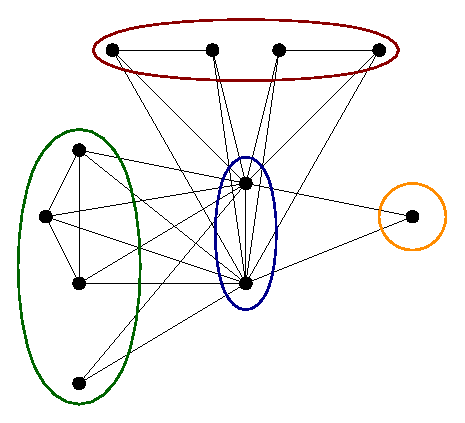
\includegraphics[width=25cm]{img/cluster-module-partition}
        \end{center}
        \vspace{1em}

        El \emph{cluster module number} $\cm(G)$ de $G$ es la mínima cantidad de conjuntos de una cluster module partition de $G$.
    }

    \block{Un poco sobre el $\cm(G)$}{
        \begin{itemize}
            \item Se puede calcular en tiempo \textbf{lineal} en el tamaño de $G$.
            \item \textbf{Generaliza} otros parámetros como el \emph{vertex cover}, \emph{twin-cover}, y \emph{neighborhood diversity}. Todo grafo que tenga alguno de esos parámetros acotados tendrá $\cm(G)$ acotado.
            \item Para cada par de conjuntos de la cluster module partition, o están \textbf{todas} las aristas entre ellos, o no hay \textbf{ninguna}.
        \end{itemize}
    }
    
    \column{0.5}
    \block{Thinness $\thin(G)$}{
        \begin{minipage}[t]{0.5\linewidth}
            \vspace{1em}
            \underline{\textbf{Solución consistente:}} dado un grafo $G$, una \emph{solución consistente} es un par $(S, \prec)$, donde
            \begin{itemize}
                \item $S$ es una partición de $V(G)$, y
                \item $\prec$ es un orden total de $V(G)$,
            \end{itemize}
            tal que para toda tripla $u \prec v \prec w$, si pasa que
            \begin{enumerate}[leftmargin=1.2cm]
                \item $u$ y $v$ pertenecen a la misma clase de $S$, y
                \item $w$ es adyacente a $u$,
            \end{enumerate}
            entonces $w$ es adyacente a $v$.
        \end{minipage}%
        \begin{adjustbox}{valign=t}
            \begin{minipage}[t]{0.5\linewidth}
                \begin{center}
                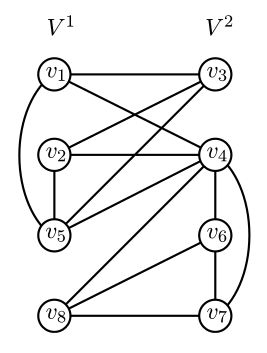
\includegraphics[width=15cm]{img/ejemplo_thinness.png}
                \end{center}
            \end{minipage}
        \end{adjustbox}


        La \emph{thinness} $\thin(G)$ de $G$ es la mínima cantidad de clases en la partición $S$ de una solución consistente $(S, \prec)$ de $G$.

        \vspace{1ex}
        {\color{gray}
        \hdashrule{36em}{4pt}{4pt}
        }

        \underline{\textbf{Lema 1:}} Si dos vértices vecinos tienen el mismo vecindario, se puede \textbf{sacar} uno sin modificar la thinness del grafo.

        \vspace{1ex}
        \underline{\textbf{Lema 2 (nuestro):}} Si tres vértices \textbf{no vecinos} tienen el mismo vecindario, se puede \textbf{sacar} uno sin modificar la thinness del grafo. 
    }

    \block{Simultaneous Interval Number $\si(G)$}{
        Una \emph{$t$-simultaneous interval representation} de un grafo $G$ es una asignación de intervalos sobre la recta y de subconjuntos de $\{1,\dots,t\}$ a cada vértice, tal que dos vértices son adyacentes si y sólo si tanto sus intervalos como sus subconjuntos se intersecan. 
        \begin{center}
            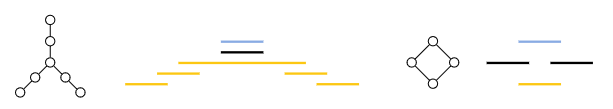
\includegraphics[width=36cm]{img/si}
        \end{center}

        El \emph{simultaneous interval number} $\si(G)$ es el mínimo natural $t$ tal que $G$ tiene una $t$-simultaneous interval representation.

        \vspace{1ex}
        {\color{gray}
        \hdashrule{36em}{4pt}{4pt}
        }

        Tanto \textsc{Thinness} como \textsc{Simultaneous Interval Number} son \textbf{NP-completos}, pero si un grafo tiene alguno de estos dos parámetros acotados, existen algoritmos \textbf{polinomiales} para muchos problemas conocidos (\textsc{Independent Set}, \textsc{$k$-Capacitated Coloring}, etc. en el caso de thinness; \textsc{Clique}, \textsc{$k$-Dominating Set}, \textsc{$k$-Independent Set}, etc. en el caso de simultaneous interval number).
    }

    % \note[
    %     targetoffsetx=-9cm, 
    %     targetoffsety=-6.5cm, 
    %     width=0.5\linewidth
    %     ]
    %     {e-mail \texttt{welcome@overleaf.com}}
\end{columns}
\block{Nuestros resultados}{
    \underline{\textbf{Teorema 1:}} Para toda clase de grafos $\mathcal{G}$ con cluster module number acotado, hay un algoritmo \textbf{polinomial} para encontrar la thinness de un grafo en $\mathcal{G}$.
    \begin{itemize}
        \item \textbf{Idea:} Encontrar una cluster module partition del grafo $G$ y aplicar lemas 1 y 2 para achicar el grafo sin cambiar la thinness a un grafo de tamaño proporcional a $\cm(G)$.
    \end{itemize}

    {\color{gray}
    \hdashrule{80cm}{4pt}{4pt}
    }

    \vspace{-1ex}
    \underline{\textbf{Teorema 2:}} Para toda clase de grafos $\mathcal{G}$ con cluster module number acotado, hay un algoritmo \textbf{polinomial} para decidir si un grafo en $\mathcal{G}$ admite una $t$-simultaneous interval representation con $t$ constante.

    {\color{gray}
    \hdashrule{80cm}{4pt}{4pt}
    }

    \vspace{-1ex}
    \underline{\textbf{Teorema 3:}} Bajo conjeturas estándar en el entorno, no existen algoritmos polinomiales que reduzcan una instancia de \textsc{Thinness} o de \textsc{Simultaneous Interval Number} a otra que tenga tamaño \textbf{polinomial} en $\p(G)$, donde $\p(G)$ puede ser treewidth, bandwidth, thinness, simultaneous interval number, etc. etc. etc\dots 
    \begin{itemize}
        \item Esto se llama un \emph{kernel}. Acá estamos diciendo que no existe \emph{kernel polinomial} para el problema \textsc{Thinness} o \textsc{Simultaneous Interval Number} \emph{parametrizado por $\p(G)$}.
    \end{itemize}
}
\end{document}